\section{三维重建技术}\label{reconstruction}
三维重建一直是学术界和工业界关注的问题,数十年来有很多相关的科研工作。
这些三维重建的方法将距离信息,如无结构化点云\cite{henry2010rgb}\cite{keller2013real}
\cite{whelan2015elasticfusion}、2.5D深度图像\cite{meilland2013unifying}或高度场\cite{gallup20103d},
转化为基于占据栅格(occupancy grids)\cite{elfes1987sensor}
或隐式曲面(implicit surfaces)的体素表达\cite{curless1996volumetric}。
在很多三维重建工作中,其默认的体素表达是TSDFs(Truncated Signed Distance Felds,
删节有向距离场)\cite{fioraio2015large}\cite{fuhrmann2014floating}。
这些基于TSDF的方法可以建立连续的曲面,系统性的处理噪声,
不需要记录显式的拓扑信息并且能够有效的做增量式的修改。
在这些方法中最有名的就是KinectFusion\cite{izadi2011kinectfusion}\cite{newcombe2011kinectfusion},
它实现了实时的相机跟踪和体素融合。

要利用相机重建三维信息,需要获得两个位置信息:物体表面和相机的相对位置以及相机在世界坐标系中的位姿。
物体和相机的相对位置可通过三维测距技术实现,相机位姿的确定则需要通过相机在每一帧中的位姿实现。
三维测距的相关工作以及在上一节介绍了,
而相机的位姿通常是基于ICP(Iterative Closest Point,迭代最近点)算法
\cite{besl1992method}及其变种实现。
这些方法会计算相邻两帧之间的相机发生的刚体变换,并将其叠加到上一帧的相机位姿上,
增量的计算相机当前的位姿。
在实际的工作中,这样的相机跟踪方法往往鲁棒性不佳,容易引入累计误差。
有很多研究这就会借助RGB图像提升每帧之间的跟踪结果\cite{whelan2013robust}
或者利用全局的位姿估计校正来提升位姿的精度。
常见的全局位姿优化方法有位姿图优化(pose graph optimization)\cite{steinbrucker2013large},
闭环检测(loop closure detection)\cite{whelan2013deformation},
增量式的BA(incremental bundle adjustement)\cite{fioraio2015large}
以及利用关键点进行或图片对相机进行重定位等。
% \begin{figure}[h]
%     \centering
%     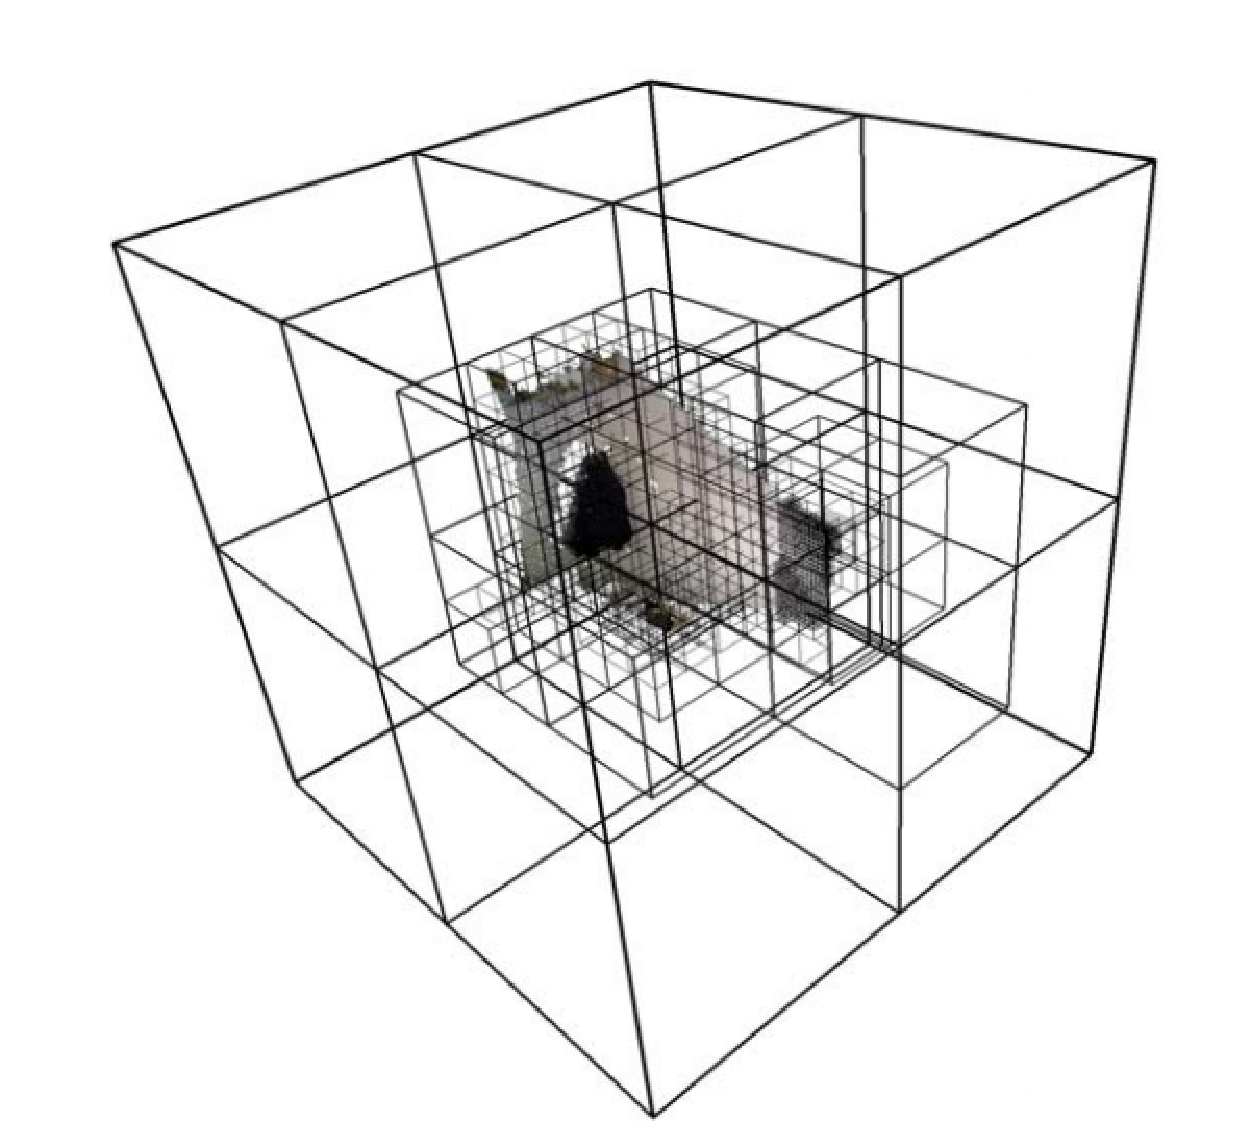
\includegraphics[width = 0.6\textwidth]{./Pictures/octree.eps}
%     \caption{八叉树结构}
%     \label{octree}
% \end{figure}

很多重建算法为了达到实时的性能,都引入了GPU并行实现。
例如KinectFusion\cite{izadi2011kinectfusion}就用GPU实现了将深度图片信息并行的融合到统一化网格的算法。
但体素信息的存储会占用大量的显存,显存大小也就成了场景分辨率的最大瓶颈。
为了突破显存对场景分辨率的限制,有的工作会将不在视野内的体素从显存中换出\cite{roth2012moving}。
Steinbrucker在2013年的工作\cite{steinbrucker2013large}采用了多尺度的八叉树(octree)数据结构
和稠密图对齐实现了大尺度室内场景的重构。
分层空间数据结构和流算法也被利用以将KinectFusion扩展到更大的场景中\cite{chen2013scalable}。
此外,还有相关的工作\cite{niessner2013real}采用体素哈希(voxel hashing)来减少分层数据结构的开销。 